\section{Organisation du Projet}

\subsection{Répartition des Tâches}

Pedro s'est chargé de la partie logicielle : déploiement de ROS 2 Jazzy sur la Raspberry Pi, développement du protocole de communication série sécurisé, calibration de la caméra et des paramètres HSV, et scripts utilitaires (télé-opération, pont série, monitoring). Luiz Felipe a pris en charge la conception physique du robot : modélisation et impression 3D du mécanisme de sondage, des bacs de batteries, de la tourelle LiDAR et des supports de capteurs, ainsi que le câblage électronique complet et le débogage des ESC. Durant la phase finale, les deux membres ont collaboré au développement du noeud principal \texttt{agri\_line\_follower}, aux tests d'intégration en laboratoire, à la campagne de validation terrain et au débogage des problèmes de communication ROS 2.

% ------------------------------------------------------------------ %
%  PHOTOS DU ROBOT - À INSÉRER (décommenter \includegraphics)
% ------------------------------------------------------------------ %
\begin{figure}[H]
    \centering
    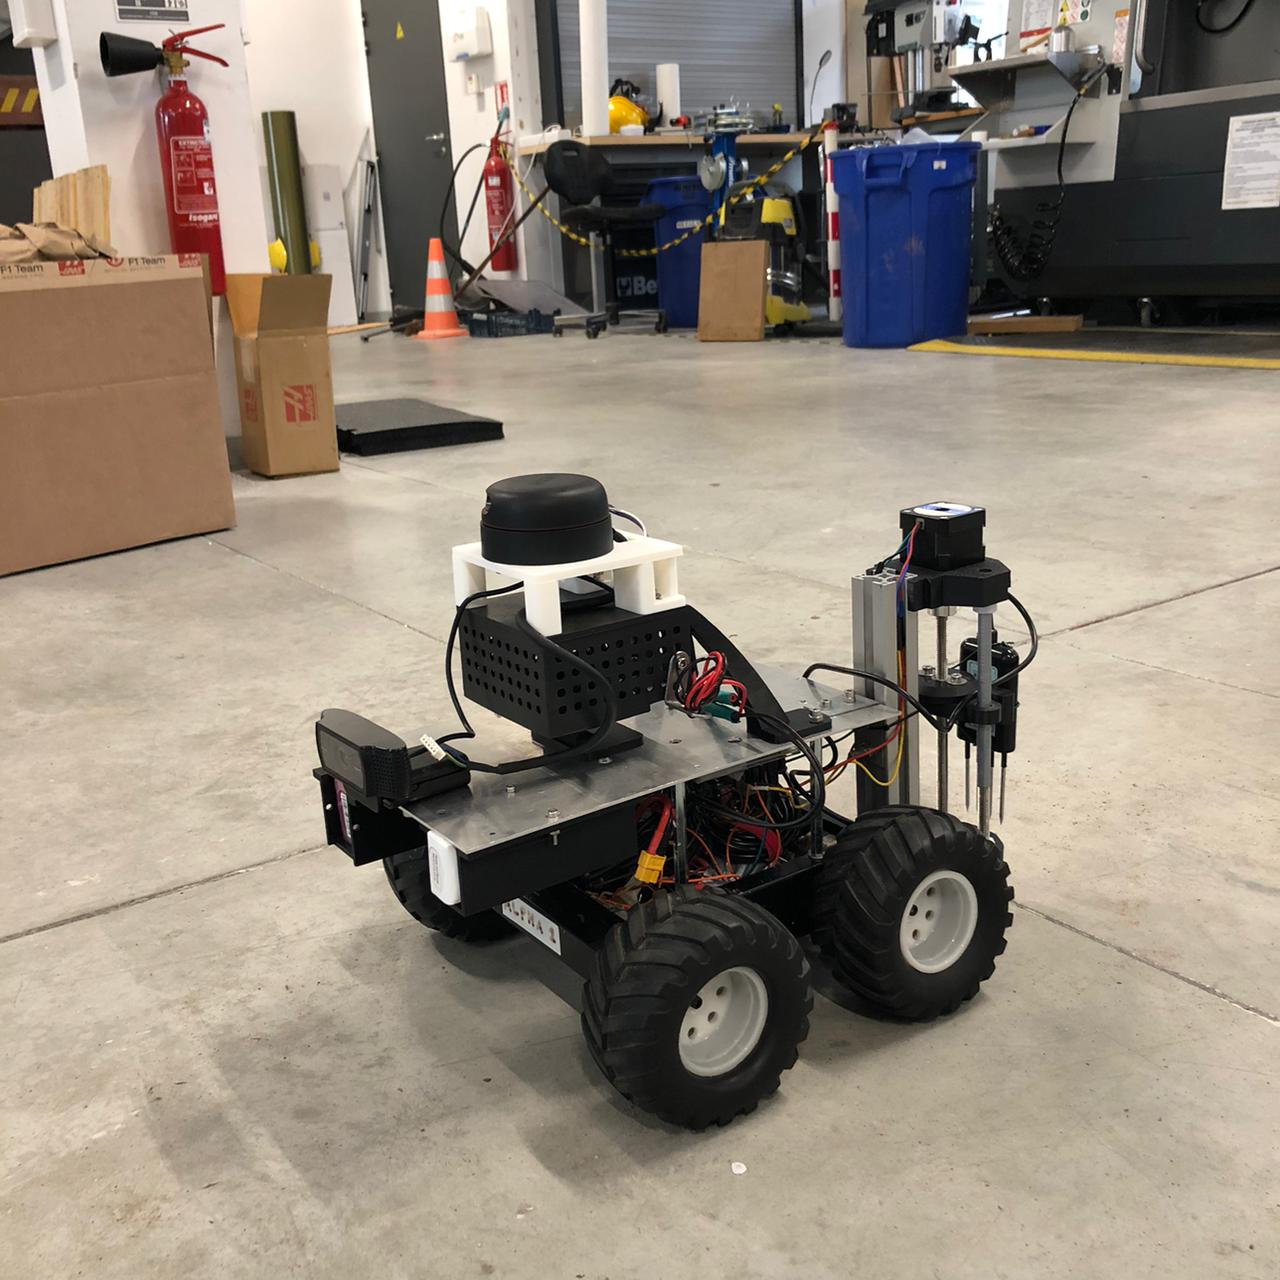
\includegraphics[width=0.85\textwidth]{images/robot.jpeg}
    \caption{Prototype AGRI-Scout finalisé : tourelle LiDAR, mécanisme de sondage et alimentation isolée.}
    \label{fig:robot_final}
\end{figure}

\begin{figure}[H]
    \centering
    \begin{minipage}{0.48\textwidth}
        \centering
        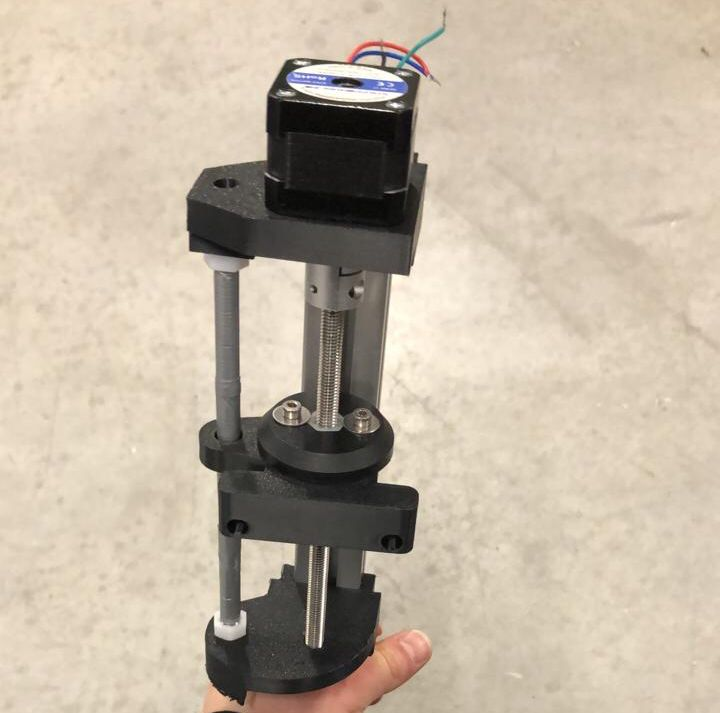
\includegraphics[width=\textwidth]{images/sonda.jpeg}
    \end{minipage}
    \hfill
    \begin{minipage}{0.48\textwidth}
        \centering
        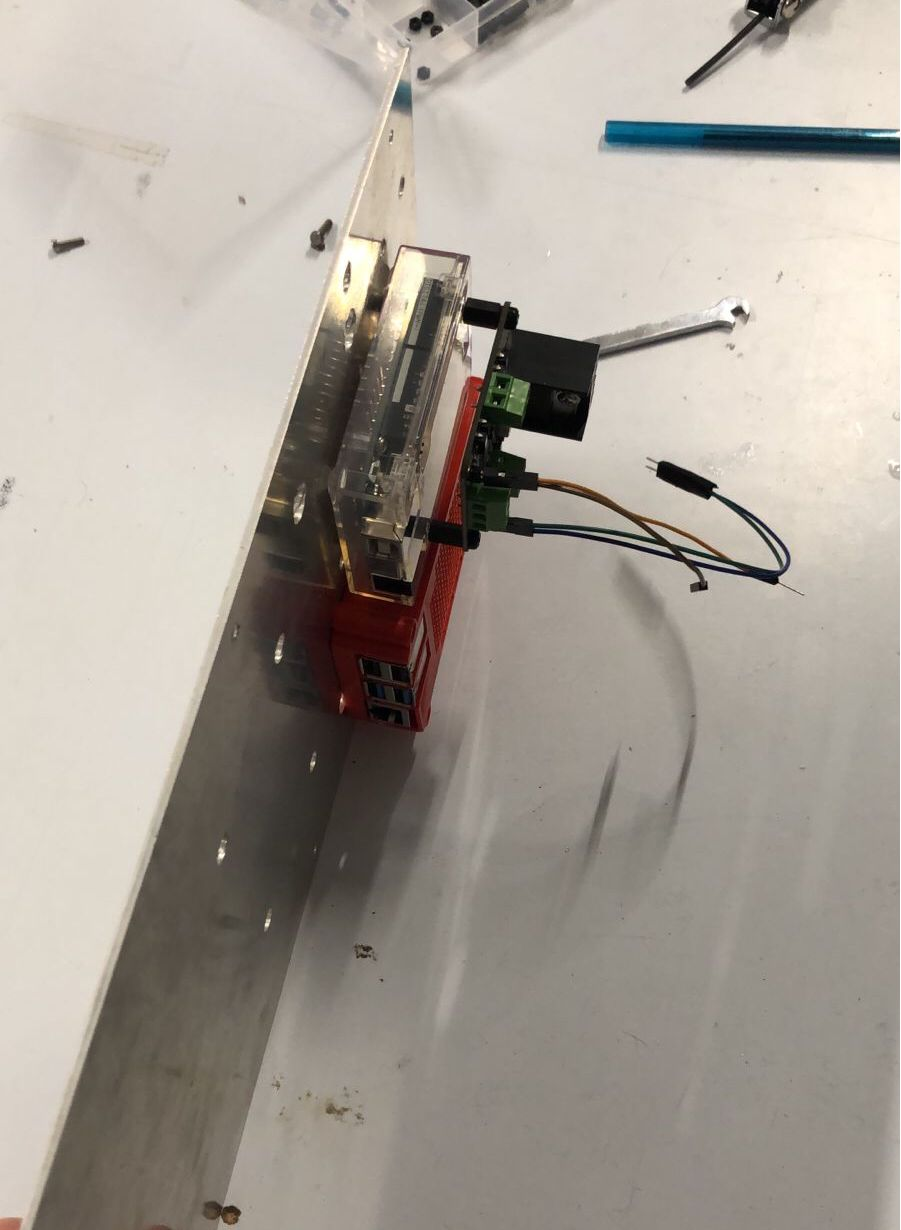
\includegraphics[angle=90, width=\textwidth]{images/pi_ino.jpeg}
    \end{minipage}
    \caption{Gauche : mécanisme de perforation 3D. Droite : architecture électronique avec isolation galvanique.}
    \label{fig:details_robot}
\end{figure}


\subsection{Chronologie du Projet (Septembre 2025 -- Avril 2026)}

Le tableau suivant retrace, mois par mois, les activités qui avaient été planifiées au démarrage du projet.

\renewcommand{\arraystretch}{1.5}
\begin{longtable}{|p{2.8cm}|p{11cm}|}
\hline
\rowcolor{headerblue!20}
\textbf{Mois} & \textbf{Activités Planifiées} \\
\hline
\endfirsthead
\hline
\rowcolor{headerblue!20}
\textbf{Mois} & \textbf{Activités Planifiées} \\
\hline
\endhead
\hline
\multicolumn{2}{r}{\textit{Suite sur la page suivante\ldots}}\\
\endfoot
\hline
\endlastfoot

\textbf{Septembre 2025}
& Définition du cahier des charges, formation de l'équipe, choix de la plateforme matérielle de base. Premiers contacts avec les composants (Arduino, ESC, LiPo). \\
\hline

\rowcolor{rowalt}
\textbf{Octobre 2025}
& Recherche bibliographique et état de l'art. Étude de l'architecture Master-Slave (RPi/Arduino). Premiers tests Arduino (PWM, lecture ultrasons). \\
\hline

\textbf{Novembre 2025}
& Assemblage mécanique préliminaire du châssis. Tests d'alimentation et dimensionnement énergétique. Premiers tests de vision (YOLO sur PC). \\
\hline

\rowcolor{rowalt}
\textbf{Décembre 2025}
& Rédaction du rapport partiel. Validation de la locomotion de base. Identification des problèmes d'alimentation (brown-outs Traco Power). Congés. \\
\hline

\textbf{Janvier 2026}
& Refonte de l'architecture d'alimentation (isolation galvanique). Migration vers USB série. Début de la conception 3D du mécanisme de sondage. Déploiement de ROS 2 Jazzy sur RPi. \\
\hline

\rowcolor{rowalt}
\textbf{Février 2026}
& Développement du noeud ROS 2 \texttt{agri\_line\_follower}. Conception du protocole de communication sécurisé. Impression 3D et assemblage des pièces mécaniques (tourelle LiDAR, bacs batteries). \\
\hline

\textbf{Mars 2026}
& Intégration du LiDAR RPLIDAR A1. Développement du watchdog logiciel. Tests d'intégration en conditions contrôlées. Calibration de la caméra. Débogage des ESC (frein ABS RC). \\
\hline

\rowcolor{rowalt}
\textbf{Avril 2026}
& Campagne de tests terrain. Validation de la mission autonome complète (suivi de ligne + sondage). Rédaction du rapport final d'avancement. \\
\hline

\end{longtable}

\subsubsection*{Problèmes ayant impacté le planning}

Plusieurs difficultés imprévues ont provoqué des décalages par rapport au planning initial. Le problème d'alimentation a été identifié tardivement et a nécessité une refonte complète de l'architecture électrique, aboutissant à trois sources isolées : une powerbank USB-C pour la Raspberry Pi, une batterie LiPo principale pour la traction, et une seconde batterie LiPo moins puissante dédiée au mécanisme de montée/descente de la sonde. Cette refonte a retardé le démarrage des développements logiciels de plusieurs semaines. La synchronisation entre Python/ROS 2 et le firmware Arduino a également demandé un travail itératif intense. Enfin, une pénurie de filament dans les imprimantes 3D du laboratoire a retardé la fabrication des pièces mécaniques, repoussant les tests finaux et la campagne de validation terrain.
